\begin{figure*}
  \centering
  \begin{subfigure}[c]{\textwidth}
    \centering
    \caption{Examples of dose-response curves with $3$ replicates}
    {\footnotesize Random} \hspace{3.85cm} {\footnotesize PLAID} \hspace{3.45cm} {\footnotesize COMPD}

    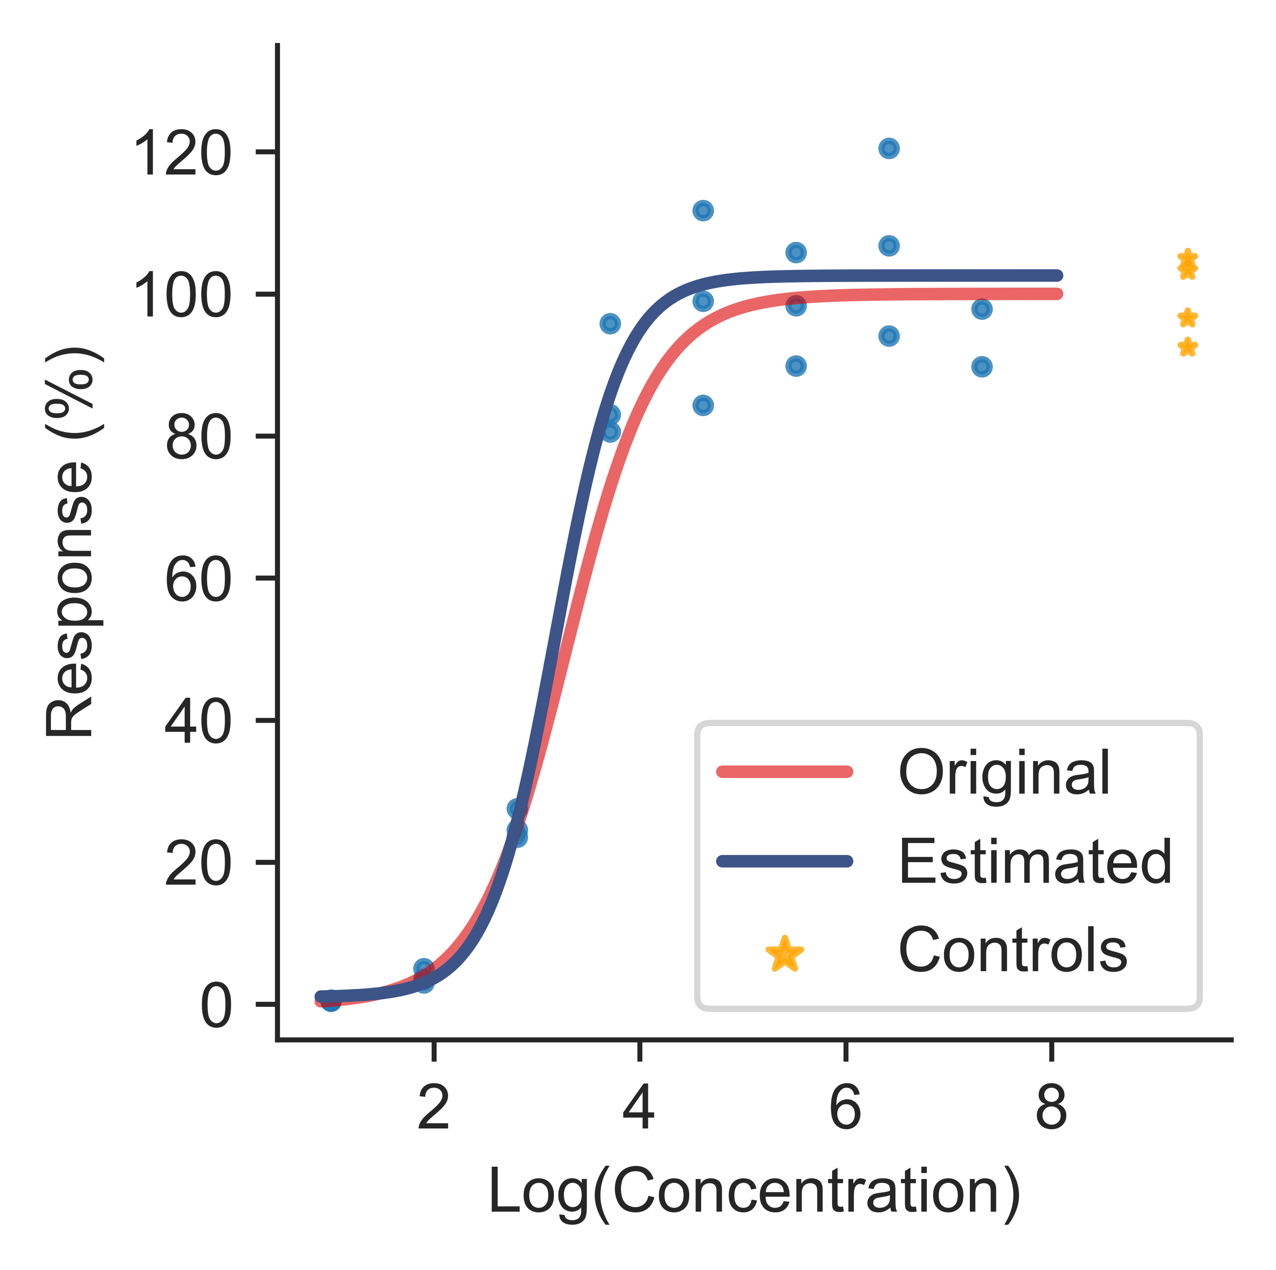
\includegraphics[width=0.3\textwidth]{figures/plate_layout_rand_02.npy_compound_4-right-half.png}
    \label{fig:dr-curves-half-right}
    \hfill
    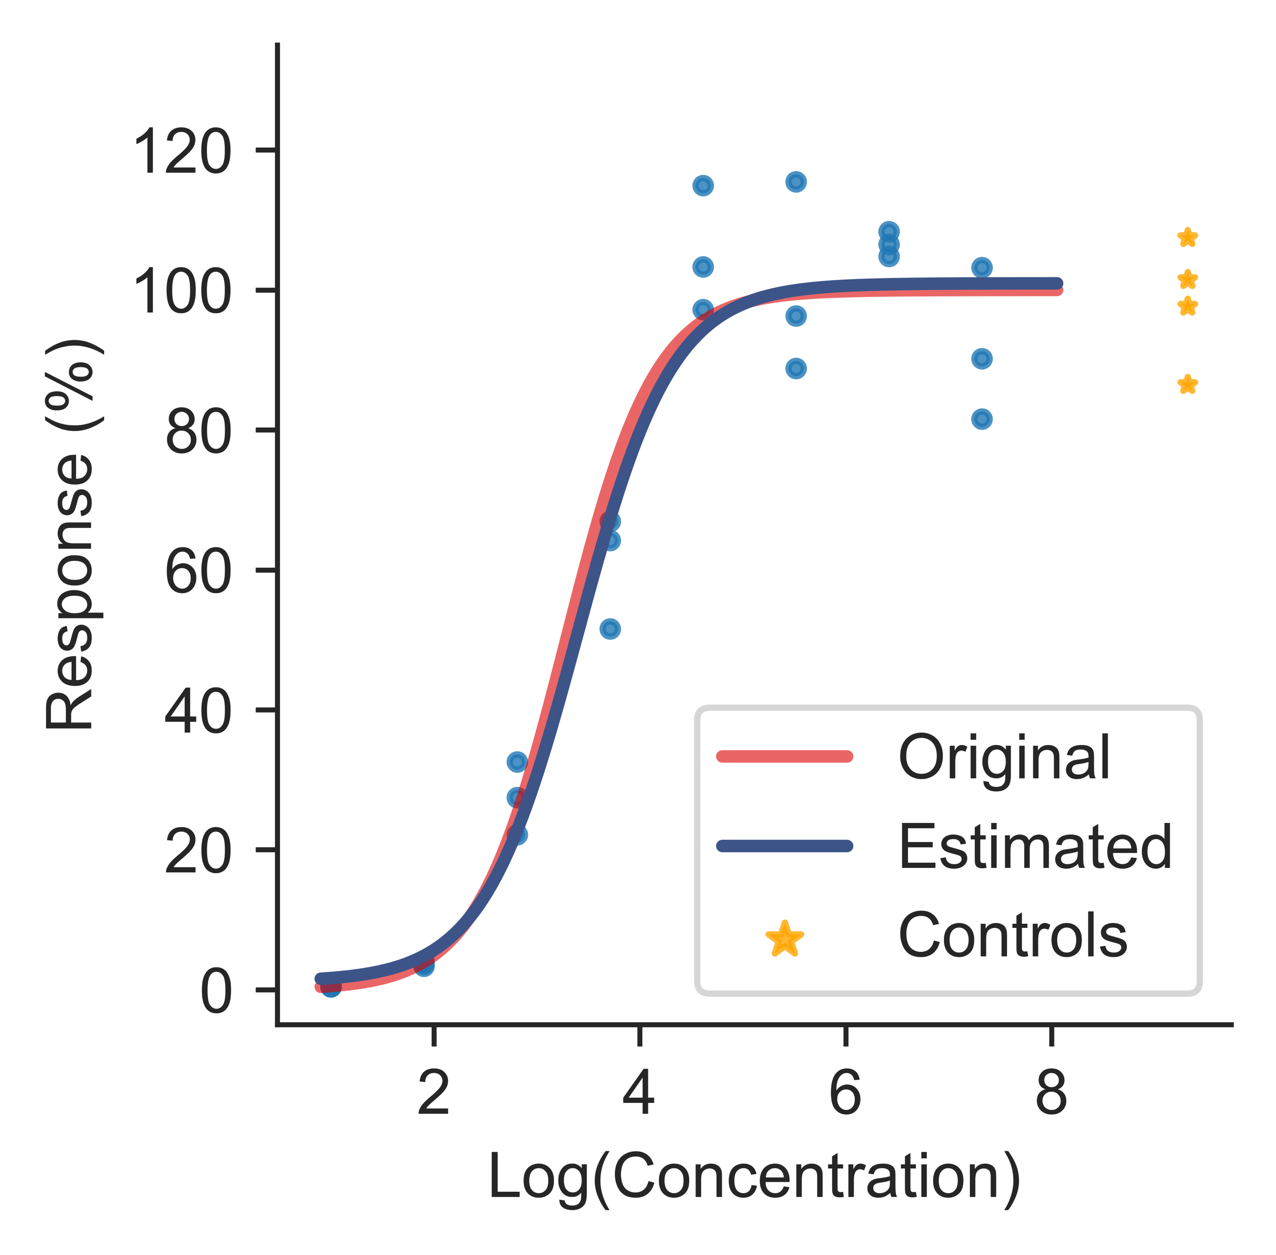
\includegraphics[width=0.3\textwidth]{figures/plate_layout_20-12-8-3_01.npy_compound_4-right-half.png}
    \hfill
    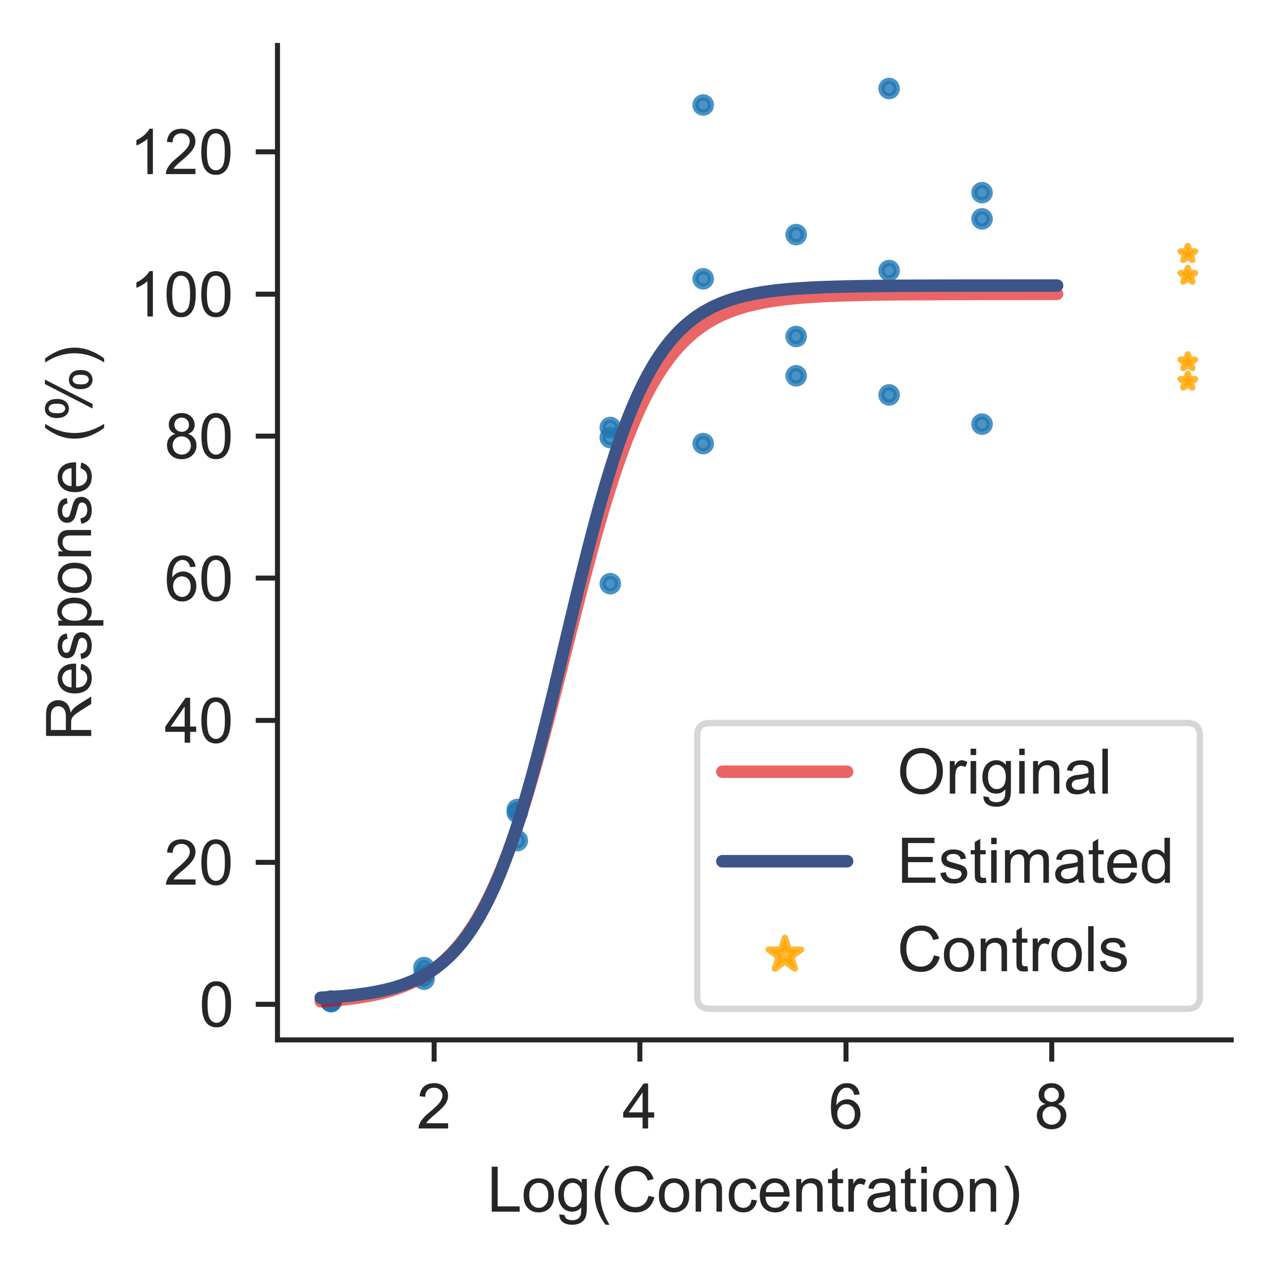
\includegraphics[width=0.3\textwidth]{figures/plate_layout_40-12-8-3_01.npy_compound_4-right-half.png}
    
  \end{subfigure}
  
  \vspace{0.3cm}

  %%%%%%%%%%%

     \begin{subfigure}[b]{0.5\textwidth}
         \centering
         \caption{Residuals}
         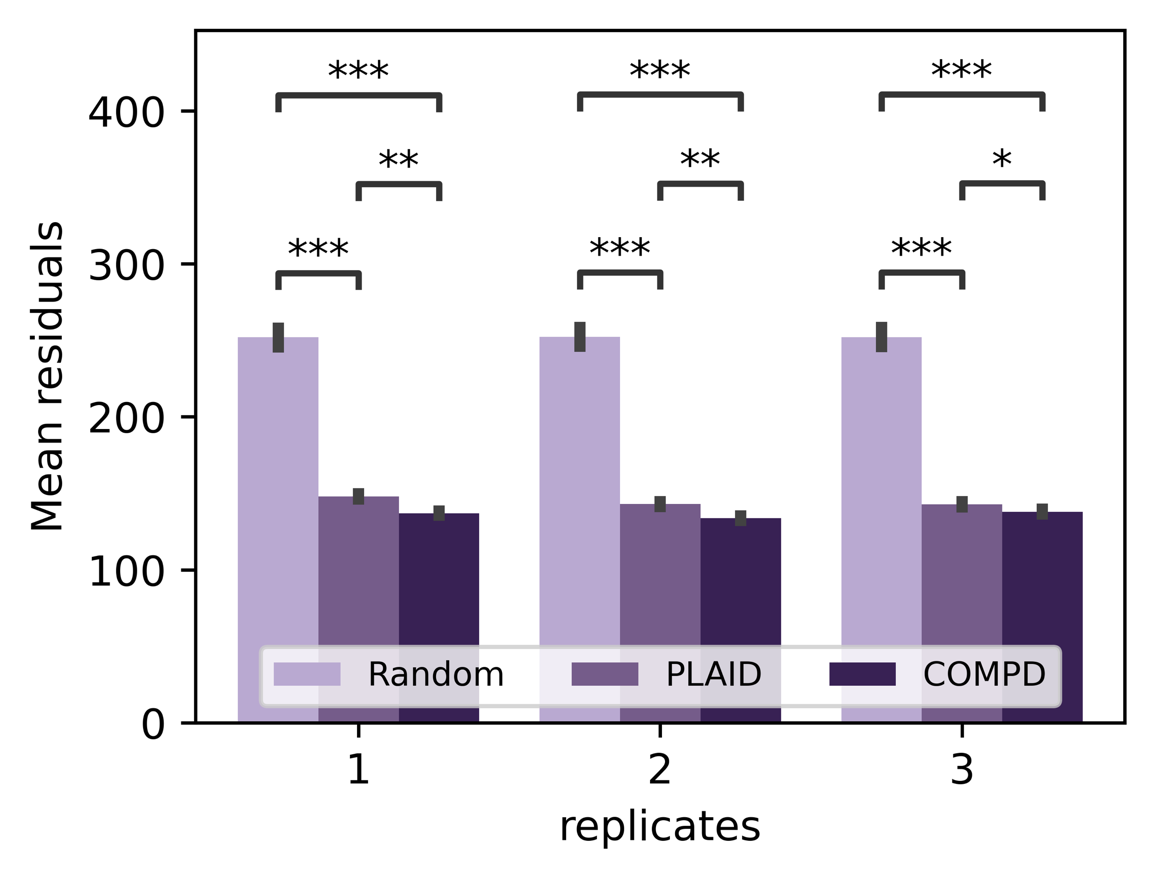
\includegraphics[width=\textwidth]{figures/residuals-1-2-3-8doses-dil8-half-columns-neg-controls-0.4_paper.png}
         \label{fig:residuals-8-doses-half-right}
       \end{subfigure}
       \hfill
       \begin{subfigure}[b]{0.49\textwidth}
         \centering
         \caption{Mean absolute d (max) difference}
         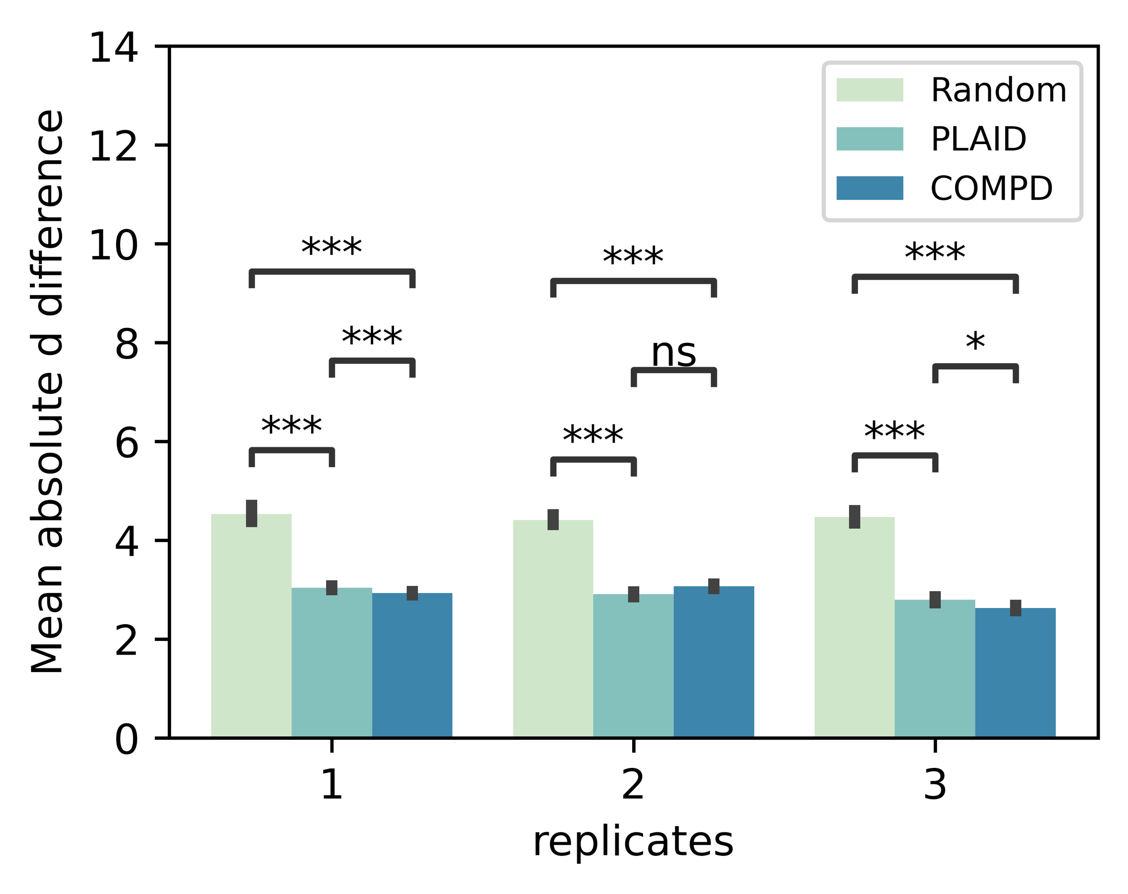
\includegraphics[width=\textwidth]{figures/dose-response-d_diff-1-2-3-8doses-dil8-right-half-neg-controls-0.4_paper.png}
       \end{subfigure}


  %%%%%%%%%%%

  
     \begin{subfigure}[c]{0.48\textwidth}
         \centering
         \caption{Relative $\text{IC}_{50}$/$\text{EC}_{50}$}
         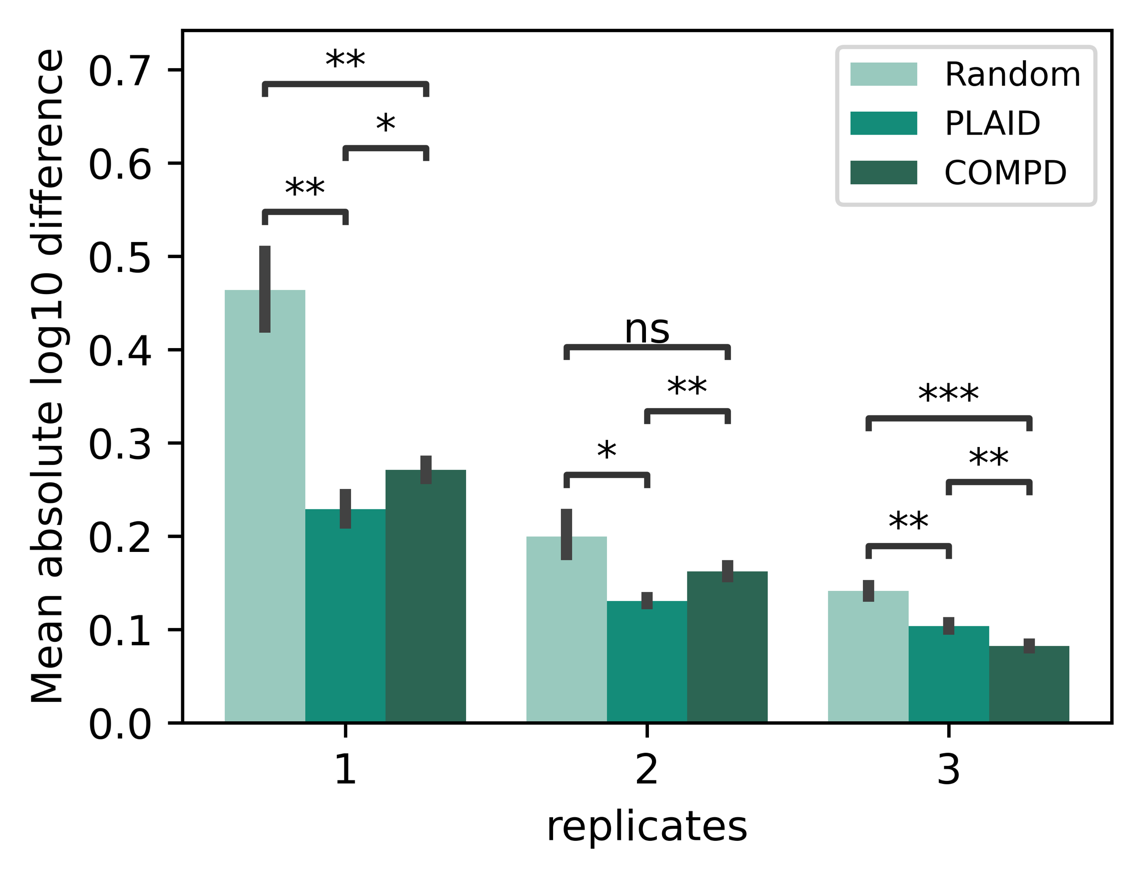
\includegraphics[width=\textwidth]{figures/dose-response-relic50-1-2-3-8doses-dil8-half-columns-neg-controls-0.4_paper.png}
         \label{fig:relic50-8-doses-half-right} 
       \end{subfigure}
       %\hfill
       \begin{subfigure}[c]{0.5\textwidth} 
         \centering
         \caption{Absolute $\text{IC}_{50}$/$\text{EC}_{50}$}
         \includegraphics[width=\textwidth]{figures/dose-response-absic50-1-2-3-8doses-dil8-right-half-neg-controls-0.4_paper.png}
         \label{fig:absic50-8-doses-half-right}
     \end{subfigure}

%%%%%
     \caption{Comparison between expected and
       obtained values for dose response curves with
       $8$ doses, $1$, $2$, or $3$ replicates, $20$ negative controls on
       384-well plate, and strong plate effects with a linear relationship to column number on the right side of the plate. %, 
       * indicates ${p<10^{-4}}$, ** indicates ${p<10^{-12}}$, ***
    indicates ${p<10^{-43}}$.}
        \label{fig:dose_response_paper}
\end{figure*}


%%% Local Variables: 
%%% mode: latex
%%% TeX-master: "main.tex"
%%% End: 


